\section{Sintonia de controladores}


\begin{frame}{Sintonia}
	\begin{block}{Introdução}
		\begin{itemize}
			\item As principais razões para a baixa performance de processos automatizados estão relacionadas ao \textbf{mau funcionamento} de válvulas, aos \textbf{sensores} e ao \textbf{ajuste incorreto} dos controladores PID.
			\item O \textbf{ajuste} (sintonia) é o trabalho de \textbf{determinar valores adequados} para \textbf{parâmetros} de um controlador, de tal modo que o processo exiba as propriedades desejadas.
			\item Apesar de \textbf{extensivos estudos} sobre esse assunto, ainda não existe um \textbf{método único} para proceder a este ajuste.
			\item Muitos controladores possuem uma função denominada \textbf{autoajuste} (self-tune) que, durante sua inicialização, a partir de um \textbf{sinal de entrada} e da \textbf{resposta obtida}, \textbf{calcula os parâmetros} do controle PID e \textbf{memoriza} os respectivos valores.
		\end{itemize}
	\end{block}
\end{frame}


\begin{frame}{Sintonia}
	\begin{block}{Introdução}
		\begin{itemize}
			\item O controlador PID possui três parâmetros de ajuste:
			\begin{enumerate}
				\item\normalsize Ganho proporcional – $ K_c $
				\item\normalsize Tempo integral – $ T_i $
				\item\normalsize Tempo derivativo – $ T_d $ 
			\end{enumerate}
			\item O projeto de um controlador nem sempre é \textbf{suficientemente completo}, e os métodos de autoajuste, por serem \textbf{genéricos}, muitas vezes fornecem ajustes que \textbf{podem ser melhorados}.
			\item Em alguns casos, nos quais os requisitos de desempenho \textbf{não são críticos}, técnicos experientes podem fazer o ajuste \textbf{manualmente} a partir de \textbf{métodos práticos} de sintonia.
		\end{itemize}
	\end{block}
\end{frame}


\begin{frame}{Sintonia}
	\begin{block}{Introdução}
		\begin{itemize}
			\item Existem vários métodos para ajustar controles em malha fechada.
			\item O mais conhecido e utilizado até hoje foi originalmente descrito formalmente por J. G. Ziegler e B. B. Nichols em 1942.
			\item Para esses autores, um ajuste ótimo apresenta um caimento de $ 1/4 $ durante o regime transitório.
		\end{itemize}
	\end{block}

	\centering
	\includegraphics[width=0.5\linewidth]{Figuras/Ch14/fig1}
\end{frame}


\begin{frame}{Tentativa e erro}
	\begin{block}{Passo a passo}		
		Um procedimento típico de sintonia de controladores PID realizado em malha fechada é o seguinte:
		\begin{enumerate}
			\item Eliminar os termos integral e derivativo escolhendo $ \bm{T_i} $ com seu valor \textbf{máximo} e $ \bm{T_d} $ com seu valor \textbf{mínimo}.
			\item Atribuir a $ \bm{K_c} $ um valor \textbf{baixo} e colocar o controlador no modo \textbf{automático}.
			\item \textbf{Aumentar} o ganho $ \bm{K_c} $, em pequenos passos, até que ocorra uma oscilação \textbf{estável}, ou seja, com amplitude \textbf{constante}.			
			\item \textbf{Reduzir}, então, $ \bm{K_c} $ pela \textbf{metade}.		
			\item \textbf{Diminuir} $ \bm{T_i} $ \textbf{gradualmente} até observar novamente a ocorrência de uma oscilação \textbf{continuada}. Fixe então $ \bm{T_i} $ em \textbf{3 vezes este valor}.
			\item \textbf{Aumentar} $ \bm{T_d} $ também gradualmente até que ocorra novamente uma \textbf{oscilação mantida}. Faça então $ \bm{T_d} $ igual a $ \bm{1/3} $ deste valor.
		\end{enumerate}
	\end{block}
\end{frame}


\begin{frame}{Tentativa e erro}
	\begin{block}{Ganho supremo}
		\begin{enumerate}
			\item O valor de $ K_c $ que se obtém no passo 3 é chamado de \textbf{ganho supremo},
			denotado por $ \bm{K_u} $.
			\item Ao realizar o procedimento anterior, é importante que a saída do controlador
			\textbf{não se sature}.
			\item Se houver saturação, pode ocorrer uma oscilação estável ainda
			que $ K_c > K_u $.
		\end{enumerate}
	\end{block}
\end{frame}


\begin{frame}{Tentativa e erro}
	\centering
	\includegraphics[width=0.7\linewidth]{Figuras/Ch14/fig2}
\end{frame}


\begin{frame}{Método de Ziegler-Nichols em malha fechada}
	\begin{block}{Introdução}
		\begin{itemize}
			\item Também conhecido como ``\textbf{segundo método de Ziegler-Nichols}'', trata-se de algo \textbf{similar à tentativa e erro}, porém mais \textbf{sistemático}.
			\item Nesse método, devemos encontrar $ K_u $ assim como descrito até o terceiro passo da tentativa e erro, assim como o \textbf{período de oscilação} do processo $ P_u $ (período crítico).
		\end{itemize}
	\end{block}

	\centering
	\includegraphics[width=0.5\linewidth]{Figuras/Ch14/fig3}
	
\end{frame}


\begin{frame}{Método de Ziegler-Nichols em malha fechada}
	\begin{block}{2º Ziegler-Nichols - Parâmetros para controladores}
		\resizebox{\textwidth}{!}{
			\begin{tabular}{cC{5em}C{5em}C{5em}}
				\toprule
				\thead{\normalsize Tipo do\\\normalsize controlador} & K_p & T_i & T_d\\ \midrule
				P & \num{0.5}\cdot K_u & - & - \\[0.2em]
				PI & \num{0.4}\cdot K_u & \num{0.8}\cdot P_u & - \\[0.2em]
				PID & \num{0.6}\cdot K_u & \num{0.5}\cdot P_u & \num{0.125}\cdot P_u \\ \bottomrule
		\end{tabular}}
	\end{block}
\end{frame}


\begin{frame}{Método de Ziegler-Nichols em malha fechada}
	\begin{block}{Exemplo \#01}
		\begin{itemize}
			\item Um técnico quer sintonizar um controlador num processo em \textbf{malha fechada} e decide usar o \textbf{2º método de Ziegler-Nichols} para tal.
			\item Primeiro faz o processo \textbf{oscilar}.
		\end{itemize}
	\end{block}
	
	\centering
	\includegraphics[width=0.55\linewidth]{Figuras/Ch14/fig3n2}
	
\end{frame}


\begin{frame}{Método de Ziegler-Nichols em malha fechada}
	\begin{block}{Exemplo \#01}
		\begin{itemize}
			\item De acordo com o programa que fornece o gráfico utilizado, $ P_u=\SI{4}{\second} $ e $ K_c=10 $ na condição de \textbf{oscilação}.
			\item Portanto, pela tabela, se deseja sintonizar um \textbf{controlador PI}, por exemplo, deve utilizar
			\begin{gather*}
			K_p=\num{0.4}\cdot K_u=\num{0.4}\cdot10=4\\
			T_i=\num{0.8}\cdot P_u=\num{0.8}\cdot4=\SI{3.2}{\second}
			\end{gather*}
		\end{itemize}
	\end{block}
\end{frame}


\begin{frame}{Sintonia em malha aberta}
	\begin{block}{Introdução - Função de transferência}
		\begin{itemize}
			\item Alguns métodos de sintonia analisam o comportamento do processo em \textbf{malha aberta}, aplicando uma \textbf{função degrau}, ou seja, que ``\textbf{pula}'' entre dois valores, por vezes de 0\% a 100\%.
			\item A partir da aplicação desse sinal e da análise da saída do processo, podemos analisar sua resposta em \textbf{curva característica} e, então, reduzí-lo à uma \textbf{função de primeiro grau com tempo morto}.
			\item Essa função trata-se de uma \textbf{função de transferência}, que é uma ferramenta analítica \textbf{muito útil} em controle.
			\item A função de transferência é uma \textbf{forma conveniente} de transcrever o \textbf{comportamento} do processo, e tem o seguinte formato:
			\[ G(s)=\dfrac{K\text{e}^{-Ls}}{Ts+1} \]
		\end{itemize}
	\end{block}
\end{frame}


\begin{frame}{Sintonia em malha aberta}
	\begin{block}{Resposta característica}
		\begin{itemize}
			\item Cada uma das constantes numa função de transferência tem um \textbf{significado físico} que pode ser encontrado no \textbf{gráfico} da \textbf{resposta característica} do processo.
		\end{itemize}
	\end{block}

	\centering
	\scalebox{1.2}{\begin{tikzpicture}[scale=0.5]
			\draw (-4,-3) rectangle (4,3); %CLP
		\draw (-4,0) -- (-2.5,0); %Div in out
		\draw (-2.5,-3) -- (-2.5,3); %Div cartoes
		\draw (-1.5,-2.5) rectangle (0,2.5); %Mem dados
		\draw (0.5,-2.5) rectangle (3.5,-1); %Mem prog
		\draw (1,0) rectangle (3,2); %CPU
		\draw (-4,-5) rectangle (4,-3); %Alimentacao
		\draw (-2.5,4) rectangle (4,6); %Term de prog
		
		\draw (1,2.6) node {CLP};
		
		\draw (-3.25,1.5) node[text width=1.5cm,align=center,rotate=90] {\small Cartões de input};
		
		\draw (-3.25,-1.5) node[text width=1.5cm,align=center,rotate=90] {\small Cartões de output};
		
		\node at (2,1) {\small CPU};
		
		\node[rotate=90,text width=1.5cm,align=center] at (-0.75,0) {\small Memória de dados};
		
		\node[text width=2cm,align=center] at (2,-1.75) {\footnotesize Memória de programa};
		
		\node at (-6,0) {Campo};
		
		\node at (0,-4) {Alimentação};
		
		\node[text width=3cm,align=center] at (0.75,5) {Terminal de programação};
		
		\draw[-Latex] (-8,1.5) -- node[above] {Entradas} +(4,0);
		\draw[Latex-] (-8,-1.5) -- node[below] {Saídas} +(4,0);
		\draw[-Latex] (-2.5,1.5) -- +(1,0);
		\draw[Latex-] (-2.5,-1.5) -- +(1,0);
		\draw[-Latex] (0,1.5) -- +(1,0);
		\draw[Latex-] (0,0.5) -- +(1,0);
		\draw[Latex-] (2,0) -- +(0,-1);
		
		\draw[-Latex] (-1.5,4) -- +(0,-1);
		\draw[Latex-] (3,4) -- +(0,-1);
	\end{tikzpicture}}
	
\end{frame}


\begin{frame}{Sintonia em malha aberta}
	\begin{block}{Constantes da função de transferência}
		\begin{itemize}
			\item $ L $ é o \textbf{tempo morto}.
			\item $ T $ é a \textbf{constante de tempo} (tempo necessário para o processo atingir \num{0.632} do valor final).
			\item $ V_f $ e $ V_i $ são os valores \textbf{final} e \textbf{inicial} do \textbf{processo} durante a aplicação do sinal em degrau.
		\end{itemize}
	\end{block}
	
	\centering
	\scalebox{1}{\begin{tikzpicture}[scale=0.5]
			\draw (-4,-3) rectangle (4,3); %CLP
		\draw (-4,0) -- (-2.5,0); %Div in out
		\draw (-2.5,-3) -- (-2.5,3); %Div cartoes
		\draw (-1.5,-2.5) rectangle (0,2.5); %Mem dados
		\draw (0.5,-2.5) rectangle (3.5,-1); %Mem prog
		\draw (1,0) rectangle (3,2); %CPU
		\draw (-4,-5) rectangle (4,-3); %Alimentacao
		\draw (-2.5,4) rectangle (4,6); %Term de prog
		
		\draw (1,2.6) node {CLP};
		
		\draw (-3.25,1.5) node[text width=1.5cm,align=center,rotate=90] {\small Cartões de input};
		
		\draw (-3.25,-1.5) node[text width=1.5cm,align=center,rotate=90] {\small Cartões de output};
		
		\node at (2,1) {\small CPU};
		
		\node[rotate=90,text width=1.5cm,align=center] at (-0.75,0) {\small Memória de dados};
		
		\node[text width=2cm,align=center] at (2,-1.75) {\footnotesize Memória de programa};
		
		\node at (-6,0) {Campo};
		
		\node at (0,-4) {Alimentação};
		
		\node[text width=3cm,align=center] at (0.75,5) {Terminal de programação};
		
		\draw[-Latex] (-8,1.5) -- node[above] {Entradas} +(4,0);
		\draw[Latex-] (-8,-1.5) -- node[below] {Saídas} +(4,0);
		\draw[-Latex] (-2.5,1.5) -- +(1,0);
		\draw[Latex-] (-2.5,-1.5) -- +(1,0);
		\draw[-Latex] (0,1.5) -- +(1,0);
		\draw[Latex-] (0,0.5) -- +(1,0);
		\draw[Latex-] (2,0) -- +(0,-1);
		
		\draw[-Latex] (-1.5,4) -- +(0,-1);
		\draw[Latex-] (3,4) -- +(0,-1);
	\end{tikzpicture}}
	
\end{frame}


\begin{frame}{Sintonia em malha aberta}
	\begin{block}{Ponto de inflexão}
		\begin{itemize}
			\item A linha a partir da qual determinamos os valores de $ L $ e $ T $ é a \textbf{extensão da tangente} no \textbf{ponto de inflexão} da curva de \textbf{resposta característica}.
			\item O \textbf{ponto de inflexão} de uma curva é o ponto exato onde a curva \textbf{muda a direção de mudança} (a variação estava crescendo e começa a diminuir).
			\item Podemos ver o ponto de inflexão, também, como o momento onde a \textbf{concavidade} da curva \textbf{se altera}.
		\end{itemize}
	\end{block}
\end{frame}


\begin{frame}{Sintonia em malha aberta}
	
	\centering
	\includegraphics[width=0.9\linewidth]{Figuras/Ch14/fig6}
	
	\bigskip
	
	Visualização do ponto de inflexão
\end{frame}


\begin{frame}{Sintonia em malha aberta}
	\begin{block}{Primeiro método de Ziegler-Nichols}
		\begin{itemize}
			\item Um dos métodos utilizados para sintonizar controladores PID em malha aberta é o método de \textbf{Ziegler-Nichols em malha aberta}, também conhecido como \textbf{primeiro método de Ziegler-Nichols}.
			\item Consiste em, usando a função de transferência, encontrar o \textbf{ganho} e \textbf{tempos} do controlador utilizando dados \textbf{tabelados}.
			\item Sendo $ \Delta X $ a variação da entrada (função degrau) e $ \Delta VP $ a variação na saída do processo: \[ K=\dfrac{\Delta VP}{\Delta X} \]
		\end{itemize}
	\end{block}
\end{frame}


\begin{frame}{Sintonia em malha aberta}
	\begin{block}{1º Ziegler-Nichols - Parâmetros para controladores}
		\resizebox{\textwidth}{!}{
			\begin{tabular}{cC{7em}C{7em}C{7em}}
				\toprule
				\thead{\normalsize Tipo do\\\normalsize controlador} & K_p & T_i & T_d\\ \midrule
				P & \dfrac{T}{KL} & - & - \\[1em]
				PI & \num{0.9}\cdot\dfrac{T}{KL} & \num{3.3}\cdot L & - \\[1em]
				PID & \num{1.2}\cdot\dfrac{T}{KL} & 2\cdot L & \num{0.5}\cdot L \\ \bottomrule
		\end{tabular}}
	\end{block}
\end{frame}


\begin{frame}{Sintonia em malha aberta}
	\begin{block}{Primeiro método de Ziegler-Nichols - Exemplo \#01}
		\begin{itemize}
			\item Suponha que, numa fábrica de cola, a mistura que dá origem ao produto final deva ficar durante \SI{40}{\second} à uma temperatura de \SI{200}{\degreeCelsius} para adquirir a consistência desejada.
			\item Para que isso ocorra sem problemas, contratam dois técnicos em automação industrial, que devem encontrar os parâmetros para o controlador de temperatura do forno das colas.
			\item Os técnicos vão utilizar o \textbf{1º método de Ziegler-Nichols} para o trabalho.
		\end{itemize}
	\end{block}
\end{frame}


\begin{frame}{Sintonia em malha aberta}
	\centering
	\includegraphics[width=0.9\linewidth]{Figuras/Ch14/fig6n2}
\end{frame}


\begin{frame}{Sintonia em malha aberta}
	\begin{block}{Primeiro método de Ziegler-Nichols - Exemplo \#01}
		\begin{itemize}
			\item A \textbf{curva característica} do processo encontrada para uma entrada $ \Delta X=5\% $ está ilustrada abaixo.
		\end{itemize}
	\end{block}
	
	\centering
	\scalebox{1.3}{

\tikzset{every picture/.style={line width=0.75pt}} %set default line width to 0.75pt        

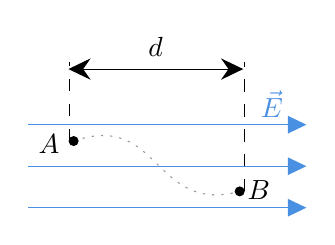
\begin{tikzpicture}[x=0.75pt,y=0.75pt,yscale=-1,xscale=1]
%uncomment if require: \path (0,300); %set diagram left start at 0, and has height of 300

%Curve Lines [id:da6177490068384819] 
\draw [color={rgb, 255:red, 155; green, 155; blue, 155 }  ,draw opacity=1 ] [dash pattern={on 0.84pt off 2.51pt}]  (137.88,127.88) .. controls (180,113.4) and (176,163.4) .. (217.88,152.13) ;


%Straight Lines [id:da7124330895115376] 
\draw [color={rgb, 255:red, 74; green, 144; blue, 226 }  ,draw opacity=1 ]   (116,120) -- (247,120) ;
\draw [shift={(250,120)}, rotate = 180] [fill={rgb, 255:red, 74; green, 144; blue, 226 }  ,fill opacity=1 ][line width=0.08]  [draw opacity=0] (8.93,-4.29) -- (0,0) -- (8.93,4.29) -- cycle    ;

%Straight Lines [id:da12792354611605283] 
\draw [color={rgb, 255:red, 74; green, 144; blue, 226 }  ,draw opacity=1 ]   (116,140) -- (247,140) ;
\draw [shift={(250,140)}, rotate = 180] [fill={rgb, 255:red, 74; green, 144; blue, 226 }  ,fill opacity=1 ][line width=0.08]  [draw opacity=0] (8.93,-4.29) -- (0,0) -- (8.93,4.29) -- cycle    ;

%Straight Lines [id:da4044562129660001] 
\draw [color={rgb, 255:red, 74; green, 144; blue, 226 }  ,draw opacity=1 ]   (116,160) -- (247,160) ;
\draw [shift={(250,160)}, rotate = 180] [fill={rgb, 255:red, 74; green, 144; blue, 226 }  ,fill opacity=1 ][line width=0.08]  [draw opacity=0] (8.93,-4.29) -- (0,0) -- (8.93,4.29) -- cycle    ;

%Shape: Circle [id:dp28224868607946574] 
\draw  [fill={rgb, 255:red, 0; green, 0; blue, 0 }  ,fill opacity=1 ] (135.75,127.88) .. controls (135.75,126.7) and (136.7,125.75) .. (137.88,125.75) .. controls (139.05,125.75) and (140,126.7) .. (140,127.88) .. controls (140,129.05) and (139.05,130) .. (137.88,130) .. controls (136.7,130) and (135.75,129.05) .. (135.75,127.88) -- cycle ;
%Shape: Circle [id:dp03942976292609046] 
\draw  [color={rgb, 255:red, 0; green, 0; blue, 0 }  ,draw opacity=1 ][fill={rgb, 255:red, 0; green, 0; blue, 0 }  ,fill opacity=1 ] (215.75,152.13) .. controls (215.75,150.95) and (216.7,150) .. (217.88,150) .. controls (219.05,150) and (220,150.95) .. (220,152.13) .. controls (220,153.3) and (219.05,154.25) .. (217.88,154.25) .. controls (216.7,154.25) and (215.75,153.3) .. (215.75,152.13) -- cycle ;
%Straight Lines [id:da5788684610773114] 
\draw  [dash pattern={on 4.5pt off 4.5pt}]  (135.75,127.88) -- (135.75,90) ;


%Straight Lines [id:da7063621547892809] 
\draw  [dash pattern={on 4.5pt off 4.5pt}]  (220,152.13) -- (220,90) ;


%Straight Lines [id:da8063380246624134] 
\draw    (138.35,93.2) -- (216.6,93.2) ;
\draw [shift={(219.6,93.2)}, rotate = 180] [fill={rgb, 255:red, 0; green, 0; blue, 0 }  ][line width=0.08]  [draw opacity=0] (10.72,-5.15) -- (0,0) -- (10.72,5.15) -- (7.12,0) -- cycle    ;
\draw [shift={(135.35,93.2)}, rotate = 0] [fill={rgb, 255:red, 0; green, 0; blue, 0 }  ][line width=0.08]  [draw opacity=0] (10.72,-5.15) -- (0,0) -- (10.72,5.15) -- (7.12,0) -- cycle    ;

% Text Node
\draw (233.4,110) node [color={rgb, 255:red, 74; green, 144; blue, 226 }  ,opacity=1 ]  {$\vec{E}$};
% Text Node
\draw (177.33,82.33) node   {$d$};
% Text Node
\draw (126,129.33) node   {$A$};
% Text Node
\draw (227.13,151.4) node   {$B$};


\end{tikzpicture}
}
	
\end{frame}


\begin{frame}{Sintonia em malha aberta}
	\begin{block}{Primeiro método de Ziegler-Nichols - Exemplo \#01}
		\begin{itemize}
			\item Utilizando \[ K=\dfrac{\Delta VP}{\Delta X}=\dfrac{51\%-45\%}{5\%}=\dfrac{6\%}{5\%}=\num{1.2} \]
			os técnicos encontram a \textbf{função de transferência de 1ª ordem} do processo \[ G(s)=\dfrac{\num{1.2}
				\text{e}^{-s}}{2s+1} \]
			\item A partir desta, podem sintonizar o \textbf{controlador PID} da fábrica, utilizando os parâmetros
			\begin{gather*}
			K_p=\num{1.2}\cdot\dfrac{T}{KL}=\num{1,2}\cdot\dfrac{2}{\num{1.2}\cdot1}=2\\
			T_i=2\cdot L=2\cdot1=\SI{2}{\second}\\
			T_d=\num{0.5}\cdot L=\num{0.5}\cdot1=\SI{0.5}{\second}
			\end{gather*}
		\end{itemize}
	\end{block}
\end{frame}


\begin{frame}{Sintonia em malha aberta}
	\begin{block}{Primeiro método de Ziegler-Nichols - Exemplo \#02}
		\begin{itemize}
			\item A \textbf{curva característica} do processo encontrada para uma entrada $ \Delta X=1 $ (degrau unitário) está ilustrada abaixo.
		\end{itemize}
	\end{block}
	
	\centering
	\includegraphics[width=0.7\linewidth]{Figuras/Ch14/fig3n3}
	
\end{frame}


\begin{frame}{Sintonia em malha aberta}
	\begin{block}{Primeiro método de Ziegler-Nichols - Exemplo \#02}
		\begin{itemize}
			\item Utilizando \[ K=\dfrac{\Delta VP}{\Delta X}=\dfrac{5-0}{1}=5 \] e fazendo $ L=\SI{0.8}{\second} $ e $ T=t_2-L=\SI{4.5}{\second}-\SI{0.8}{\second}=\SI{3.7}{\second} $
			temos \[ G(s)=\dfrac{5
				\text{e}^{-\num{0.8}s}}{\num{3.7}s+1} \]
			\item A partir desta, um \textbf{controlador PI} pode ser sintonizado utilizando os parâmetros
			\begin{gather*}
			K_p=\num{0.9}\cdot\dfrac{T}{KL}=\num{0.9}\cdot\dfrac{\num{3.7}}{\num{5}\cdot\num{0.8}}=\num{0.9}\cdot\num{0.925}=\num{0.8325}\\
			T_i=\num{3.3}\cdot L=\num{3.3}\cdot\num{0.8}=\SI{2.64}{\second}
			\end{gather*}
		\end{itemize}
	\end{block}
\end{frame}


\begin{frame}{Sintonia em malha aberta}
	\begin{block}{Método de Cohen-Coon}
		\begin{itemize}
			\item O método de sintonia \textbf{Cohen-Coon} é \textbf{mais geral} do que o de Ziegler-Nichols em malha aberta.
			\item Ziegler-Nichols funciona somente para processos onde o tempo morto é \textbf{metade} da constante de tempo.
			\item Cohen-Coon consegue transpor essa dificuldade, podendo se estender mais até do que com o tempo morto sendo o \textbf{dobro} da constante de tempo.
			\item O método Cohen-Coon também é capaz de sintonizar controladores PD.
		\end{itemize}
	\end{block}
\end{frame}


\begin{frame}{Sintonia em malha aberta}
	\begin{block}{Constantes da função de transferência}
		\begin{itemize}
			\item No método Cohen-Coon devemos encontrar as constantes da função de transferência através dos valores abaixo.
		\end{itemize}
	\end{block}
	
	\centering
	\scalebox{1.5}{

\tikzset{every picture/.style={line width=0.75pt}} %set default line width to 0.75pt        

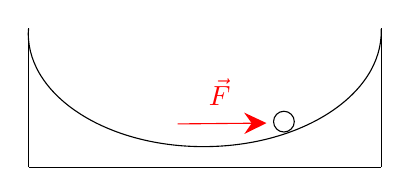
\begin{tikzpicture}[x=0.75pt,y=0.75pt,yscale=-1,xscale=1]
%uncomment if require: \path (0,300); %set diagram left start at 0, and has height of 300

%Straight Lines [id:da3398984480833569] 
\draw    (90,103) -- (90,170) ;


%Straight Lines [id:da39213437306955434] 
\draw    (260,103) -- (260,170) ;


%Straight Lines [id:da7536538469625644] 
\draw    (90,170) -- (260,170) ;


%Shape: Arc [id:dp6883804097522237] 
\draw  [draw opacity=0] (260,103) .. controls (260,103) and (259.87,104.01) .. (259.88,104.37) .. controls (260.12,134.75) and (222.24,159.67) .. (175.28,160.04) .. controls (128.31,160.41) and (90.05,136.08) .. (89.81,105.71) .. controls (89.81,105.53) and (89.81,105.35) .. (89.81,105.17) -- (174.84,105.04) -- cycle ; \draw   (259.85,103.29) .. controls (259.87,103.65) and (259.87,104.01) .. (259.88,104.37) .. controls (260.12,134.75) and (222.24,159.67) .. (175.28,160.04) .. controls (128.31,160.41) and (90.05,136.08) .. (89.81,105.71) .. controls (89.81,105.53) and (90,103) .. (90,103) ;
%Shape: Circle [id:dp54266808828771] 
\draw   (208,148) .. controls (208,145.24) and (210.24,143) .. (213,143) .. controls (215.76,143) and (218,145.24) .. (218,148) .. controls (218,150.76) and (215.76,153) .. (213,153) .. controls (210.24,153) and (208,150.76) .. (208,148) -- cycle ;
%Straight Lines [id:da8066991195909812] 
\draw [color={rgb, 255:red, 255; green, 0; blue, 0 }  ,draw opacity=1 ]   (161.8,149.1) -- (202.6,148.72) ;
\draw [shift={(204.6,148.7)}, rotate = 539.46] [fill={rgb, 255:red, 255; green, 0; blue, 0 }  ,fill opacity=1 ][line width=0.75]  [draw opacity=0] (10.72,-5.15) -- (0,0) -- (10.72,5.15) -- (7.12,0) -- cycle    ;


% Text Node
\draw (120,147) node  [align=left] {};
% Text Node
\draw (182,133.8) node [color={rgb, 255:red, 255; green, 0; blue, 0 }  ,opacity=1 ]  {$\vec{F}$};


\end{tikzpicture}
}
	
\end{frame}


\begin{frame}{Sintonia em malha aberta}
	\begin{block}{Constantes da função de transferência}
		\begin{itemize}
			\item $ T=\dfrac{3}{2}\del{t_2-t_1} $.
			\item $ L=t_2-T $
		\end{itemize}
	\end{block}
	
	\centering
	\scalebox{1.4}{

\tikzset{every picture/.style={line width=0.75pt}} %set default line width to 0.75pt        

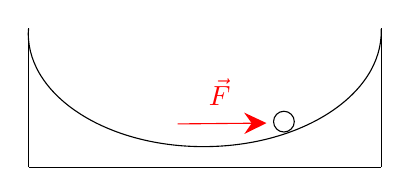
\begin{tikzpicture}[x=0.75pt,y=0.75pt,yscale=-1,xscale=1]
%uncomment if require: \path (0,300); %set diagram left start at 0, and has height of 300

%Straight Lines [id:da3398984480833569] 
\draw    (90,103) -- (90,170) ;


%Straight Lines [id:da39213437306955434] 
\draw    (260,103) -- (260,170) ;


%Straight Lines [id:da7536538469625644] 
\draw    (90,170) -- (260,170) ;


%Shape: Arc [id:dp6883804097522237] 
\draw  [draw opacity=0] (260,103) .. controls (260,103) and (259.87,104.01) .. (259.88,104.37) .. controls (260.12,134.75) and (222.24,159.67) .. (175.28,160.04) .. controls (128.31,160.41) and (90.05,136.08) .. (89.81,105.71) .. controls (89.81,105.53) and (89.81,105.35) .. (89.81,105.17) -- (174.84,105.04) -- cycle ; \draw   (259.85,103.29) .. controls (259.87,103.65) and (259.87,104.01) .. (259.88,104.37) .. controls (260.12,134.75) and (222.24,159.67) .. (175.28,160.04) .. controls (128.31,160.41) and (90.05,136.08) .. (89.81,105.71) .. controls (89.81,105.53) and (90,103) .. (90,103) ;
%Shape: Circle [id:dp54266808828771] 
\draw   (208,148) .. controls (208,145.24) and (210.24,143) .. (213,143) .. controls (215.76,143) and (218,145.24) .. (218,148) .. controls (218,150.76) and (215.76,153) .. (213,153) .. controls (210.24,153) and (208,150.76) .. (208,148) -- cycle ;
%Straight Lines [id:da8066991195909812] 
\draw [color={rgb, 255:red, 255; green, 0; blue, 0 }  ,draw opacity=1 ]   (161.8,149.1) -- (202.6,148.72) ;
\draw [shift={(204.6,148.7)}, rotate = 539.46] [fill={rgb, 255:red, 255; green, 0; blue, 0 }  ,fill opacity=1 ][line width=0.75]  [draw opacity=0] (10.72,-5.15) -- (0,0) -- (10.72,5.15) -- (7.12,0) -- cycle    ;


% Text Node
\draw (120,147) node  [align=left] {};
% Text Node
\draw (182,133.8) node [color={rgb, 255:red, 255; green, 0; blue, 0 }  ,opacity=1 ]  {$\vec{F}$};


\end{tikzpicture}
}
\end{frame}


\begin{frame}{Sintonia em malha aberta}
	\begin{block}{Cohen-Coon - Parâmetros para controladores}
		\centering
		\begin{adjustbox}{totalheight=0.89\textheight-2\baselineskip}
			\begin{tabular}{cC{5em}C{5em}C{5em}}
				\toprule
				\thead{\normalsize Tipo do\\\normalsize controlador} & K_p & T_i & T_d\\ \midrule
				P 	& \dfrac{T}{KL}\del{1+\dfrac{L}{3T}} & - & - \\[0.5em]
				PI 	& \dfrac{T}{KL}\del{\num{0.9}+\dfrac{L}{12T}} & L\del{\dfrac{30+\dfrac{3L}{T}}{9+\dfrac{20L}{T}}} & - \\[0.5em]
				PD	& \dfrac{T}{KL}\del{\num{1.25}+\dfrac{L}{6T}} & - & L\del{\dfrac{6-\dfrac{2L}{T}}{22+\dfrac{3L}{T}}} \\[2em]
				PID & \dfrac{T}{KL}\del{\num{1.33}+\dfrac{L}{4T}} & L\del{\dfrac{32+\dfrac{6L}{T}}{13+\dfrac{8L}{T}}} & L\del{\dfrac{4}{11+\dfrac{2L}{T}}} \\ \bottomrule
			\end{tabular}
		\end{adjustbox}
	\end{block}
\end{frame}


\begin{frame}{Sintonia em malha aberta}
	\begin{block}{Método de Cohen-Coon - Exemplo \#01}
		\begin{itemize}
			\item Uma máquina de pintura de automóveis deve ter seu \textbf{controlador PD} sintonizado, para isso o técnico da fábrica utiliza o \textbf{método de Cohen-Coon}.
			\item Aplicando uma entrada $ \Delta X=12\% $, encontra o seguinte gráfico.
		\end{itemize}
	\end{block}
	
	\centering
	\scalebox{1.3}{

\tikzset{every picture/.style={line width=0.75pt}} %set default line width to 0.75pt        

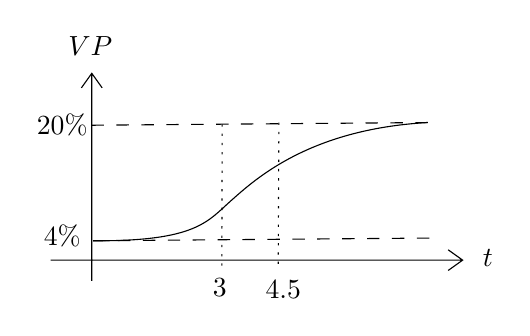
\begin{tikzpicture}[x=0.75pt,y=0.75pt,yscale=-1,xscale=1]
%uncomment if require: \path (0,300); %set diagram left start at 0, and has height of 300

%Shape: Axis 2D [id:dp8434144691544803] 
\draw  (171.87,196) -- (370.4,196)(191.72,106) -- (191.72,206) (363.4,191) -- (370.4,196) -- (363.4,201) (186.72,113) -- (191.72,106) -- (196.72,113)  ;
%Curve Lines [id:da3393494842698659] 
\draw    (192.33,186.67) .. controls (242.17,187) and (247.5,177.33) .. (258.83,167.33) .. controls (270.17,157.33) and (296.17,133) .. (353.17,129.73) ;


%Straight Lines [id:da6828905031101673] 
\draw  [dash pattern={on 4.5pt off 4.5pt}]  (191.6,131) -- (358,129.67) ;


%Straight Lines [id:da012395283086218845] 
\draw  [dash pattern={on 4.5pt off 4.5pt}]  (192.33,186.67) -- (358.73,185.33) ;


%Straight Lines [id:da9569907625895342] 
\draw  [dash pattern={on 0.84pt off 2.51pt}]  (281.87,129.73) -- (281.54,197.98) ;


%Straight Lines [id:da25982411660347404] 
\draw  [dash pattern={on 0.84pt off 2.51pt}]  (254.53,130.53) -- (254.39,200.06) ;


%%Straight Lines [id:da022260850258795317] 
%\draw    (160.2,170.6) -- (253.8,170.6) ;
%
%
%%Straight Lines [id:da5039184027623409] 
%\draw [line width=0.75]    (161,149.4) -- (282.6,149.4) ;



% Text Node
\draw (382.6,195.2) node   {$t$};
% Text Node
\draw (191,93) node   {$VP$};
% Text Node
\draw (177.5,131) node   {$20\%$};
% Text Node
\draw (177.5,184.5) node   {$4\%$};
% Text Node
\draw (253.4,209) node   {\SI{3}{\second}};
% Text Node
\draw (284,210) node   {\SI{4.5}{\second}};
%% Text Node
%\draw (135,145.5) node   {$0.632VP$};
%% Text Node
%\draw (135,168.5) node   {$0.283VP$};


\end{tikzpicture}
}
\end{frame}


\begin{frame}{Sintonia em malha aberta}
	\centering
	\includegraphics[width=0.9\linewidth]{Figuras/Ch14/fig6n3}
\end{frame}


\begin{frame}{Sintonia em malha aberta}
	\begin{block}{Método de Cohen-Coon - Exemplo \#01}
		\begin{itemize}
			\item $ T=\dfrac{3}{2}\del{\SI{4.5}{\second}-\SI{3}{\second}}=\dfrac{3}{2}\cdot\SI{1.5}{\second}=\SI{2.25}{\second} $.
			\item $ L=\SI{4.5}{\second}-\SI{2.25}{\second}=\SI{2.25}{\second} $
		\end{itemize}
	\end{block}
	
	\centering
	\scalebox{1.4}{

\tikzset{every picture/.style={line width=0.75pt}} %set default line width to 0.75pt        

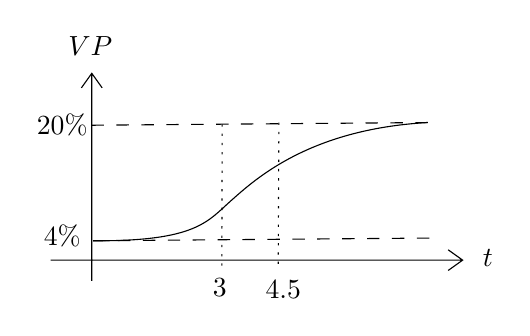
\begin{tikzpicture}[x=0.75pt,y=0.75pt,yscale=-1,xscale=1]
%uncomment if require: \path (0,300); %set diagram left start at 0, and has height of 300

%Shape: Axis 2D [id:dp8434144691544803] 
\draw  (171.87,196) -- (370.4,196)(191.72,106) -- (191.72,206) (363.4,191) -- (370.4,196) -- (363.4,201) (186.72,113) -- (191.72,106) -- (196.72,113)  ;
%Curve Lines [id:da3393494842698659] 
\draw    (192.33,186.67) .. controls (242.17,187) and (247.5,177.33) .. (258.83,167.33) .. controls (270.17,157.33) and (296.17,133) .. (353.17,129.73) ;


%Straight Lines [id:da6828905031101673] 
\draw  [dash pattern={on 4.5pt off 4.5pt}]  (191.6,131) -- (358,129.67) ;


%Straight Lines [id:da012395283086218845] 
\draw  [dash pattern={on 4.5pt off 4.5pt}]  (192.33,186.67) -- (358.73,185.33) ;


%Straight Lines [id:da9569907625895342] 
\draw  [dash pattern={on 0.84pt off 2.51pt}]  (281.87,129.73) -- (281.54,197.98) ;


%Straight Lines [id:da25982411660347404] 
\draw  [dash pattern={on 0.84pt off 2.51pt}]  (254.53,130.53) -- (254.39,200.06) ;


%%Straight Lines [id:da022260850258795317] 
%\draw    (160.2,170.6) -- (253.8,170.6) ;
%
%
%%Straight Lines [id:da5039184027623409] 
%\draw [line width=0.75]    (161,149.4) -- (282.6,149.4) ;



% Text Node
\draw (382.6,195.2) node   {$t$};
% Text Node
\draw (191,93) node   {$VP$};
% Text Node
\draw (177.5,131) node   {$20\%$};
% Text Node
\draw (177.5,184.5) node   {$4\%$};
% Text Node
\draw (253.4,209) node   {\SI{3}{\second}};
% Text Node
\draw (284,210) node   {\SI{4.5}{\second}};
%% Text Node
%\draw (135,145.5) node   {$0.632VP$};
%% Text Node
%\draw (135,168.5) node   {$0.283VP$};


\end{tikzpicture}
}
\end{frame}


\begin{frame}{Sintonia em malha aberta}
	\begin{block}{Método de Cohen-Coon - Exemplo \#01}
		\begin{itemize}
			\item Fazendo
			\[ K=\dfrac{\Delta VP}{\Delta X}=\dfrac{20\%-4\%}{12\%}=\num{1.3} \]
			temos
			\[ G(s)=\dfrac{\num{1.3}\text{e}^{-\num{2.25}s}}{\num{2.25}s+1} \]
			\item Utilizando a tabela, o controlador PD deve ser sintonizado com os parâmetros
			\begin{align*}
				K_p	&=\dfrac{T}{KL}\del{\num{1.25}+\dfrac{L}{6T}}\\
					&=\dfrac{\cancel{\num{2.25}}}{\num{1.3}\cdot\cancel{\num{2.25}}}\del{\num{1.25}+\dfrac{\cancel{\num{2.25}}}{6\cdot\cancel{\num{2.25}}}}\\
					&=\num{0.75}\del{\num{1.25}+\num{0.167}}\\
					&=\num{0.75}\cdot\num{1.417}=\num{1.0625}
			\end{align*}
		\end{itemize}
	\end{block}
\end{frame}


\begin{frame}{Sintonia em malha aberta}
	\begin{block}{Método de Cohen-Coon - Exemplo \#01}
		\begin{align*}
		T_d	&=L\del{\dfrac{6-\dfrac{2L}{T}}{22+\dfrac{3L}{T}}}\\
		&=\num{2.25}\del{\dfrac{6-\dfrac{2\cdot\cancel{\num{2.25}}}{\cancel{\num{2.25}}}}{22+\dfrac{3\cdot\cancel{\num{2.25}}}{\cancel{\num{2.25}}}}}\\
		&=\num{2.25}\del{\dfrac{6-2}{22+3}}\\
		&=\num{2.25}\cdot\num{0.16}\\
		&=\SI{0.36}{\second}
		\end{align*}
	\end{block}
\end{frame}


\frame{
	\frametitle{Exercícios}
	\begin{block}{}
		01. Determinado processo é descrito pela função de transferência abaixo. Calcule os parâmetros de um \textbf{controlador PI} de acordo com método de Cohen-Coon. \[ G(s)=\dfrac{2\text{e}^{-6s}}{12s+1} \]
		
%		\vspace{0.5cm}
		
		02. Numa indústria, a partir do gráfico abaixo, um técnico encontrou parâmetros para um \textbf{controlador PD}, explique por que isso é impossível e descreva um método para fazê-lo.
	\end{block}

	\centering
	\includegraphics[width=0.4\linewidth]{Figuras/Ch14/fig3n2}
}


\frame{
	\frametitle{Exercícios}
	\begin{block}{}
		03. Dada uma entrada em degrau de $ \Delta X=3\% $, utilizando o gráfico abaixo, encontre os parâmetros de um \textbf{controlador PI}.
		
		\vspace{0.3cm}
		
		04. Dados $ K_c=3 $ e $ P_u=\SI{0.5}{\second} $, encontre os parâmetros de um \textbf{controlador PID}.
	\end{block}
	
	\centering
	\scalebox{1.2}{

\tikzset{every picture/.style={line width=0.75pt}} %set default line width to 0.75pt        

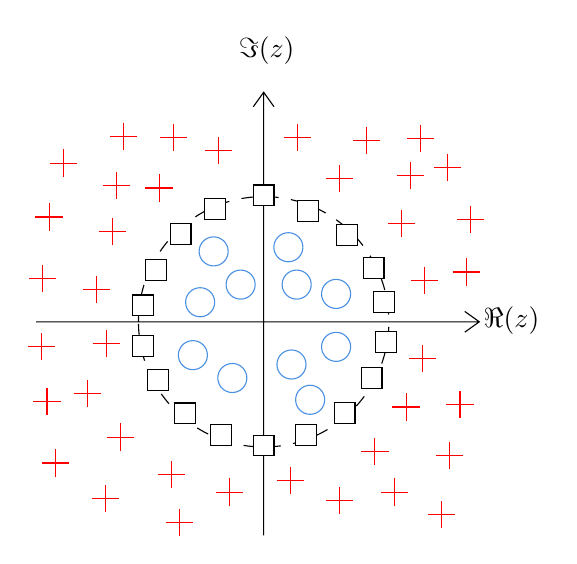
\begin{tikzpicture}[x=0.75pt,y=0.75pt,yscale=-1,xscale=1]
%uncomment if require: \path (0,300); %set diagram left start at 0, and has height of 300

%Shape: Circle [id:dp8434328262509021] 
\draw  [dash pattern={on 4.5pt off 4.5pt}] (89.28,160.6) .. controls (89.28,127.29) and (116.29,100.28) .. (149.6,100.28) .. controls (182.91,100.28) and (209.92,127.29) .. (209.92,160.6) .. controls (209.92,193.91) and (182.91,220.92) .. (149.6,220.92) .. controls (116.29,220.92) and (89.28,193.91) .. (89.28,160.6) -- cycle ;
%Shape: Axis 2D [id:dp27678030181731494] 
\draw  (40,160.6) -- (253.5,160.6)(149.6,50) -- (149.6,263.5) (246.5,155.6) -- (253.5,160.6) -- (246.5,165.6) (144.6,57) -- (149.6,50) -- (154.6,57)  ;
%Shape: Square [id:dp29640104318485094] 
\draw  [fill={rgb, 255:red, 255; green, 255; blue, 255 }  ,fill opacity=1 ] (183.6,199.6) -- (193.6,199.6) -- (193.6,209.6) -- (183.6,209.6) -- cycle ;
%Shape: Square [id:dp5015049228757054] 
\draw  [fill={rgb, 255:red, 255; green, 255; blue, 255 }  ,fill opacity=1 ] (166.1,102.2) -- (176.1,102.2) -- (176.1,112.2) -- (166.1,112.2) -- cycle ;
%Shape: Square [id:dp5724308304859749] 
\draw  [fill={rgb, 255:red, 255; green, 255; blue, 255 }  ,fill opacity=1 ] (144.6,94.7) -- (154.6,94.7) -- (154.6,104.7) -- (144.6,104.7) -- cycle ;
%Shape: Square [id:dp8722658997981245] 
\draw  [fill={rgb, 255:red, 255; green, 255; blue, 255 }  ,fill opacity=1 ] (184.6,113.7) -- (194.6,113.7) -- (194.6,123.7) -- (184.6,123.7) -- cycle ;
%Shape: Square [id:dp035501458242915174] 
\draw  [fill={rgb, 255:red, 255; green, 255; blue, 255 }  ,fill opacity=1 ] (165.1,210.2) -- (175.1,210.2) -- (175.1,220.2) -- (165.1,220.2) -- cycle ;
%Shape: Square [id:dp23226558696093957] 
\draw  [fill={rgb, 255:red, 255; green, 255; blue, 255 }  ,fill opacity=1 ] (144.6,215.2) -- (154.6,215.2) -- (154.6,225.2) -- (144.6,225.2) -- cycle ;
%Shape: Square [id:dp09667812864869552] 
\draw  [fill={rgb, 255:red, 255; green, 255; blue, 255 }  ,fill opacity=1 ] (106.6,199.7) -- (116.6,199.7) -- (116.6,209.7) -- (106.6,209.7) -- cycle ;
\draw  [color={rgb, 255:red, 255; green, 0; blue, 0 }  ,draw opacity=1 ] (159.17,71.63) -- (172.25,71.63)(165.71,65.08) -- (165.71,78.17) ;
%Shape: Circle [id:dp476022910470574] 
\draw  [color={rgb, 255:red, 74; green, 144; blue, 226 }  ,draw opacity=1 ] (118.5,126.67) .. controls (118.5,122.8) and (121.63,119.67) .. (125.5,119.67) .. controls (129.37,119.67) and (132.5,122.8) .. (132.5,126.67) .. controls (132.5,130.53) and (129.37,133.67) .. (125.5,133.67) .. controls (121.63,133.67) and (118.5,130.53) .. (118.5,126.67) -- cycle ;
\draw  [color={rgb, 255:red, 255; green, 0; blue, 0 }  ,draw opacity=1 ] (179.67,91.63) -- (192.75,91.63)(186.21,85.08) -- (186.21,98.17) ;
\draw  [color={rgb, 255:red, 255; green, 0; blue, 0 }  ,draw opacity=1 ] (209.67,113.13) -- (222.75,113.13)(216.21,106.58) -- (216.21,119.67) ;
\draw  [color={rgb, 255:red, 255; green, 0; blue, 0 }  ,draw opacity=1 ] (220.67,140.63) -- (233.75,140.63)(227.21,134.08) -- (227.21,147.17) ;
\draw  [color={rgb, 255:red, 255; green, 0; blue, 0 }  ,draw opacity=1 ] (219.67,178.13) -- (232.75,178.13)(226.21,171.58) -- (226.21,184.67) ;
\draw  [color={rgb, 255:red, 255; green, 0; blue, 0 }  ,draw opacity=1 ] (237.67,200.63) -- (250.75,200.63)(244.21,194.08) -- (244.21,207.17) ;
\draw  [color={rgb, 255:red, 255; green, 0; blue, 0 }  ,draw opacity=1 ] (232.67,225.13) -- (245.75,225.13)(239.21,218.58) -- (239.21,231.67) ;
\draw  [color={rgb, 255:red, 255; green, 0; blue, 0 }  ,draw opacity=1 ] (156.17,237.13) -- (169.25,237.13)(162.71,230.58) -- (162.71,243.67) ;
\draw  [color={rgb, 255:red, 255; green, 0; blue, 0 }  ,draw opacity=1 ] (126.67,242.63) -- (139.75,242.63)(133.21,236.08) -- (133.21,249.17) ;
\draw  [color={rgb, 255:red, 255; green, 0; blue, 0 }  ,draw opacity=1 ] (98.67,234.13) -- (111.75,234.13)(105.21,227.58) -- (105.21,240.67) ;
\draw  [color={rgb, 255:red, 255; green, 0; blue, 0 }  ,draw opacity=1 ] (74.17,216.13) -- (87.25,216.13)(80.71,209.58) -- (80.71,222.67) ;
\draw  [color={rgb, 255:red, 255; green, 0; blue, 0 }  ,draw opacity=1 ] (36.17,172.63) -- (49.25,172.63)(42.71,166.08) -- (42.71,179.17) ;
\draw  [color={rgb, 255:red, 255; green, 0; blue, 0 }  ,draw opacity=1 ] (62.67,145.13) -- (75.75,145.13)(69.21,138.58) -- (69.21,151.67) ;
\draw  [color={rgb, 255:red, 255; green, 0; blue, 0 }  ,draw opacity=1 ] (70.17,117.13) -- (83.25,117.13)(76.71,110.58) -- (76.71,123.67) ;
\draw  [color={rgb, 255:red, 255; green, 0; blue, 0 }  ,draw opacity=1 ] (46.67,84.13) -- (59.75,84.13)(53.21,77.58) -- (53.21,90.67) ;
\draw  [color={rgb, 255:red, 255; green, 0; blue, 0 }  ,draw opacity=1 ] (121.17,78.13) -- (134.25,78.13)(127.71,71.58) -- (127.71,84.67) ;
%Shape: Square [id:dp4796258381107217] 
\draw  [fill={rgb, 255:red, 255; green, 255; blue, 255 }  ,fill opacity=1 ] (197.6,129.7) -- (207.6,129.7) -- (207.6,139.7) -- (197.6,139.7) -- cycle ;
%Shape: Square [id:dp9590843867357357] 
\draw  [fill={rgb, 255:red, 255; green, 255; blue, 255 }  ,fill opacity=1 ] (202.6,146.2) -- (212.6,146.2) -- (212.6,156.2) -- (202.6,156.2) -- cycle ;
%Shape: Square [id:dp964054149374244] 
\draw  [fill={rgb, 255:red, 255; green, 255; blue, 255 }  ,fill opacity=1 ] (203.6,165.2) -- (213.6,165.2) -- (213.6,175.2) -- (203.6,175.2) -- cycle ;
%Shape: Square [id:dp7382656558458347] 
\draw  [fill={rgb, 255:red, 255; green, 255; blue, 255 }  ,fill opacity=1 ] (196.6,182.7) -- (206.6,182.7) -- (206.6,192.7) -- (196.6,192.7) -- cycle ;
%Shape: Square [id:dp21604742505805397] 
\draw  [fill={rgb, 255:red, 255; green, 255; blue, 255 }  ,fill opacity=1 ] (124.1,210.2) -- (134.1,210.2) -- (134.1,220.2) -- (124.1,220.2) -- cycle ;
%Shape: Square [id:dp8253346408417206] 
\draw  [fill={rgb, 255:red, 255; green, 255; blue, 255 }  ,fill opacity=1 ] (93.6,183.7) -- (103.6,183.7) -- (103.6,193.7) -- (93.6,193.7) -- cycle ;
%Shape: Square [id:dp3602080753175103] 
\draw  [fill={rgb, 255:red, 255; green, 255; blue, 255 }  ,fill opacity=1 ] (86.6,167.2) -- (96.6,167.2) -- (96.6,177.2) -- (86.6,177.2) -- cycle ;
%Shape: Square [id:dp7299074290585237] 
\draw  [fill={rgb, 255:red, 255; green, 255; blue, 255 }  ,fill opacity=1 ] (86.6,147.7) -- (96.6,147.7) -- (96.6,157.7) -- (86.6,157.7) -- cycle ;
%Shape: Square [id:dp3870669064913592] 
\draw  [fill={rgb, 255:red, 255; green, 255; blue, 255 }  ,fill opacity=1 ] (92.6,130.7) -- (102.6,130.7) -- (102.6,140.7) -- (92.6,140.7) -- cycle ;
%Shape: Square [id:dp0778563841598956] 
\draw  [fill={rgb, 255:red, 255; green, 255; blue, 255 }  ,fill opacity=1 ] (104.6,113.2) -- (114.6,113.2) -- (114.6,123.2) -- (104.6,123.2) -- cycle ;
%Shape: Square [id:dp4833937813802225] 
\draw  [fill={rgb, 255:red, 255; green, 255; blue, 255 }  ,fill opacity=1 ] (121.1,101.2) -- (131.1,101.2) -- (131.1,111.2) -- (121.1,111.2) -- cycle ;
%Shape: Circle [id:dp22437252791244577] 
\draw  [color={rgb, 255:red, 74; green, 144; blue, 226 }  ,draw opacity=1 ] (154.5,124.67) .. controls (154.5,120.8) and (157.63,117.67) .. (161.5,117.67) .. controls (165.37,117.67) and (168.5,120.8) .. (168.5,124.67) .. controls (168.5,128.53) and (165.37,131.67) .. (161.5,131.67) .. controls (157.63,131.67) and (154.5,128.53) .. (154.5,124.67) -- cycle ;
%Shape: Circle [id:dp4682090317035761] 
\draw  [color={rgb, 255:red, 74; green, 144; blue, 226 }  ,draw opacity=1 ] (177.5,147.17) .. controls (177.5,143.3) and (180.63,140.17) .. (184.5,140.17) .. controls (188.37,140.17) and (191.5,143.3) .. (191.5,147.17) .. controls (191.5,151.03) and (188.37,154.17) .. (184.5,154.17) .. controls (180.63,154.17) and (177.5,151.03) .. (177.5,147.17) -- cycle ;
%Shape: Circle [id:dp006880258312718768] 
\draw  [color={rgb, 255:red, 74; green, 144; blue, 226 }  ,draw opacity=1 ] (177.5,172.67) .. controls (177.5,168.8) and (180.63,165.67) .. (184.5,165.67) .. controls (188.37,165.67) and (191.5,168.8) .. (191.5,172.67) .. controls (191.5,176.53) and (188.37,179.67) .. (184.5,179.67) .. controls (180.63,179.67) and (177.5,176.53) .. (177.5,172.67) -- cycle ;
%Shape: Circle [id:dp6362725623770331] 
\draw  [color={rgb, 255:red, 74; green, 144; blue, 226 }  ,draw opacity=1 ] (156,181.17) .. controls (156,177.3) and (159.13,174.17) .. (163,174.17) .. controls (166.87,174.17) and (170,177.3) .. (170,181.17) .. controls (170,185.03) and (166.87,188.17) .. (163,188.17) .. controls (159.13,188.17) and (156,185.03) .. (156,181.17) -- cycle ;
%Shape: Circle [id:dp80425166884741] 
\draw  [color={rgb, 255:red, 74; green, 144; blue, 226 }  ,draw opacity=1 ] (158.5,142.67) .. controls (158.5,138.8) and (161.63,135.67) .. (165.5,135.67) .. controls (169.37,135.67) and (172.5,138.8) .. (172.5,142.67) .. controls (172.5,146.53) and (169.37,149.67) .. (165.5,149.67) .. controls (161.63,149.67) and (158.5,146.53) .. (158.5,142.67) -- cycle ;
%Shape: Circle [id:dp5115888880559238] 
\draw  [color={rgb, 255:red, 74; green, 144; blue, 226 }  ,draw opacity=1 ] (131.5,142.67) .. controls (131.5,138.8) and (134.63,135.67) .. (138.5,135.67) .. controls (142.37,135.67) and (145.5,138.8) .. (145.5,142.67) .. controls (145.5,146.53) and (142.37,149.67) .. (138.5,149.67) .. controls (134.63,149.67) and (131.5,146.53) .. (131.5,142.67) -- cycle ;
%Shape: Circle [id:dp9193079828474959] 
\draw  [color={rgb, 255:red, 74; green, 144; blue, 226 }  ,draw opacity=1 ] (112,151.17) .. controls (112,147.3) and (115.13,144.17) .. (119,144.17) .. controls (122.87,144.17) and (126,147.3) .. (126,151.17) .. controls (126,155.03) and (122.87,158.17) .. (119,158.17) .. controls (115.13,158.17) and (112,155.03) .. (112,151.17) -- cycle ;
%Shape: Circle [id:dp33233029245659296] 
\draw  [color={rgb, 255:red, 74; green, 144; blue, 226 }  ,draw opacity=1 ] (108.5,176.67) .. controls (108.5,172.8) and (111.63,169.67) .. (115.5,169.67) .. controls (119.37,169.67) and (122.5,172.8) .. (122.5,176.67) .. controls (122.5,180.53) and (119.37,183.67) .. (115.5,183.67) .. controls (111.63,183.67) and (108.5,180.53) .. (108.5,176.67) -- cycle ;
%Shape: Circle [id:dp3198604312654221] 
\draw  [color={rgb, 255:red, 74; green, 144; blue, 226 }  ,draw opacity=1 ] (127.5,187.67) .. controls (127.5,183.8) and (130.63,180.67) .. (134.5,180.67) .. controls (138.37,180.67) and (141.5,183.8) .. (141.5,187.67) .. controls (141.5,191.53) and (138.37,194.67) .. (134.5,194.67) .. controls (130.63,194.67) and (127.5,191.53) .. (127.5,187.67) -- cycle ;
%Shape: Circle [id:dp5700084778547776] 
\draw  [color={rgb, 255:red, 74; green, 144; blue, 226 }  ,draw opacity=1 ] (165,198.17) .. controls (165,194.3) and (168.13,191.17) .. (172,191.17) .. controls (175.87,191.17) and (179,194.3) .. (179,198.17) .. controls (179,202.03) and (175.87,205.17) .. (172,205.17) .. controls (168.13,205.17) and (165,202.03) .. (165,198.17) -- cycle ;
\draw  [color={rgb, 255:red, 255; green, 0; blue, 0 }  ,draw opacity=1 ] (240.67,136.63) -- (253.75,136.63)(247.21,130.08) -- (247.21,143.17) ;
\draw  [color={rgb, 255:red, 255; green, 0; blue, 0 }  ,draw opacity=1 ] (242.67,111.13) -- (255.75,111.13)(249.21,104.58) -- (249.21,117.67) ;
\draw  [color={rgb, 255:red, 255; green, 0; blue, 0 }  ,draw opacity=1 ] (231.67,86.13) -- (244.75,86.13)(238.21,79.58) -- (238.21,92.67) ;
\draw  [color={rgb, 255:red, 255; green, 0; blue, 0 }  ,draw opacity=1 ] (213.67,90.13) -- (226.75,90.13)(220.21,83.58) -- (220.21,96.67) ;
\draw  [color={rgb, 255:red, 255; green, 0; blue, 0 }  ,draw opacity=1 ] (192.67,73.13) -- (205.75,73.13)(199.21,66.58) -- (199.21,79.67) ;
\draw  [color={rgb, 255:red, 255; green, 0; blue, 0 }  ,draw opacity=1 ] (218.67,72.13) -- (231.75,72.13)(225.21,65.58) -- (225.21,78.67) ;
\draw  [color={rgb, 255:red, 255; green, 0; blue, 0 }  ,draw opacity=1 ] (99.67,71.63) -- (112.75,71.63)(106.21,65.08) -- (106.21,78.17) ;
\draw  [color={rgb, 255:red, 255; green, 0; blue, 0 }  ,draw opacity=1 ] (92.67,96.13) -- (105.75,96.13)(99.21,89.58) -- (99.21,102.67) ;
\draw  [color={rgb, 255:red, 255; green, 0; blue, 0 }  ,draw opacity=1 ] (36.67,139.63) -- (49.75,139.63)(43.21,133.08) -- (43.21,146.17) ;
\draw  [color={rgb, 255:red, 255; green, 0; blue, 0 }  ,draw opacity=1 ] (72.17,95.13) -- (85.25,95.13)(78.71,88.58) -- (78.71,101.67) ;
\draw  [color={rgb, 255:red, 255; green, 0; blue, 0 }  ,draw opacity=1 ] (75.67,71.13) -- (88.75,71.13)(82.21,64.58) -- (82.21,77.67) ;
\draw  [color={rgb, 255:red, 255; green, 0; blue, 0 }  ,draw opacity=1 ] (39.67,110.13) -- (52.75,110.13)(46.21,103.58) -- (46.21,116.67) ;
\draw  [color={rgb, 255:red, 255; green, 0; blue, 0 }  ,draw opacity=1 ] (58.17,195.13) -- (71.25,195.13)(64.71,188.58) -- (64.71,201.67) ;
\draw  [color={rgb, 255:red, 255; green, 0; blue, 0 }  ,draw opacity=1 ] (102.67,257.13) -- (115.75,257.13)(109.21,250.58) -- (109.21,263.67) ;
\draw  [color={rgb, 255:red, 255; green, 0; blue, 0 }  ,draw opacity=1 ] (66.67,245.63) -- (79.75,245.63)(73.21,239.08) -- (73.21,252.17) ;
\draw  [color={rgb, 255:red, 255; green, 0; blue, 0 }  ,draw opacity=1 ] (42.67,228.63) -- (55.75,228.63)(49.21,222.08) -- (49.21,235.17) ;
\draw  [color={rgb, 255:red, 255; green, 0; blue, 0 }  ,draw opacity=1 ] (38.67,199.13) -- (51.75,199.13)(45.21,192.58) -- (45.21,205.67) ;
\draw  [color={rgb, 255:red, 255; green, 0; blue, 0 }  ,draw opacity=1 ] (67.17,171.13) -- (80.25,171.13)(73.71,164.58) -- (73.71,177.67) ;
\draw  [color={rgb, 255:red, 255; green, 0; blue, 0 }  ,draw opacity=1 ] (206.17,242.63) -- (219.25,242.63)(212.71,236.08) -- (212.71,249.17) ;
\draw  [color={rgb, 255:red, 255; green, 0; blue, 0 }  ,draw opacity=1 ] (228.67,253.63) -- (241.75,253.63)(235.21,247.08) -- (235.21,260.17) ;
\draw  [color={rgb, 255:red, 255; green, 0; blue, 0 }  ,draw opacity=1 ] (196.67,223.13) -- (209.75,223.13)(203.21,216.58) -- (203.21,229.67) ;
\draw  [color={rgb, 255:red, 255; green, 0; blue, 0 }  ,draw opacity=1 ] (211.67,201.63) -- (224.75,201.63)(218.21,195.08) -- (218.21,208.17) ;
\draw  [color={rgb, 255:red, 255; green, 0; blue, 0 }  ,draw opacity=1 ] (179.67,246.63) -- (192.75,246.63)(186.21,240.08) -- (186.21,253.17) ;

% Text Node
\draw (151,30) node   {$\Im(z)$};
% Text Node
\draw (269,160) node   {$\Re(z)$};


\end{tikzpicture}
}
}


\section*{Referências}
\frame{
	\frametitle{Referências e Exercícios Complementares}
	\begin{itemize}
		\item BAYER, Fernando Mariano; ARAÚJO, Olinto César Bassi de. Controle Automático de Processos, 3 ed. UFSM : Colégio Técnico Industrial de Santa Maria, 2011.
	\end{itemize}
	%\centering{\alert{Página 546 - \textbf{Capítulo 6}}} \\
	%\centering{\alert{Lista de exercícios 01}}
}